\documentclass[deposito, acronym, symbols]{fei}

%\usepackage{glossaries}
\usepackage{subcaption} 
\usepackage{float}
%\usepackage{units}
\usepackage[portuguese]{algorithm2e}
\usepackage{biblatex}
\usepackage{amsmath}
\usepackage{listings}
\lstset{frame=tb,
language=Matlab,
aboveskip=3mm,
belowskip=3mm,
showstringspaces=false,
columns=flexible,
basicstyle={\small\ttfamily},
numbers=left,
numberstyle=\tiny\color{gray},
keywordstyle=\color{blue},
commentstyle=\color{dkgreen},
stringstyle=\color{mauve},
breaklines=true,
breakatwhitespace=true,
tabsize=4,
frame=shadowbox,
literate= {á}{{\'a}}1 {â}{{\^a}}1 {ã}{{\~a}}1 {é}{{\'e}}1 {ê}{\^e}1 {ç}{\c{c}}1 {í}{\i}1 {ú}{\'u}1 {ó}{{\'o}}1 {ô}{{\^o}}1 {õ}{{\~o}}1 {Á}{{\'A}}1 {É}{{\'E}}1, }
%%
\usepackage{color}
\definecolor{dkgreen}{rgb}{0,0.6,0}
\definecolor{mauve}{rgb}{0.58,0,0.82}
\usepackage[utf8]{inputenc}
\usepackage{chngcntr} %Faz com que o numero das notas de rodape aumente crescentemente.
\usepackage{appendix}
\counterwithout{footnote}{chapter}% "
\usepackage{siunitx}
\sisetup{output-exponent-marker=\ensuremath{\mathrm{e}}} %Escrita que precede cada entrada na lista de ilustrações.
\renewcommand{\cftfigurepresnum}{Figura }
\setlength{\cftfigurenumwidth}{5.7em}

\usepackage{titling}

%\makeglossaries
%%\newacronym[] {achpt} {ACT} {Aparecido ChupeTão}

\newacronym[longplural=Associações Brasileiras de Normas Técnicas]{abnt}{ABNT}{Associação Brasileira de Normas Técnicas}

\newacronym{ibge}{IBGE}{Instituto Brasileiro de Geografia e Estatística}

\newacronym{ashrae}{ASHRAE}{\textit{American Society of Heating, Refrigerating and Air-Conditioning Engineers}}

\newacronym{nbr}{NBR}{Norma Brasileira}

\newacronym{pmv}{PMV}{\textit{Predicted Mean Vote}}
	
\newacronym{ppd}{PPD}{\textit{Predicted Percentage of Dissatisfied}}
		
\newacronym{vgd}{VGD}{Ventilação Geral Diluidor}
		
\newacronym{vgl}{VGL}{Ventilação Local Exaustora}
		
\newacronym{cfd}{CFD}{\textit{Computational Fluid Dynamics}}
		
\newacronym{pcb}{PCB}{\textit{Printed Circuit Board}}
		
\newacronym{sms}{SMS}{\textit{Short Message Service}}
		
%\newglossaryentry{pi}{parent=greek,type=symbols,name={\ensuremath{\pi}},sort=p,description={número irracional que representa [razão entre a circunferência de qualquer círculo e seu diâmetro]}}
		


\title{Análises de uma estrutura 2D com elementos se comportando como viga e pórtico e arranjo de dados}
\author{ Felipe Estevão Coquito de Mello \\ Gabriel Mola da Silva \\ Netuno Trindade Torrente Rovaroto \\ Vitoria Fedatto Stefaneli}
\cidade{São Bernardo do Campo}
\instituicao{Centro Universitário FEI}

\addbibresource{Referencias.bib}
%\bibliographystyle{plain}
\bibliography{Referencias}
\graphicspath{ {Imagens/}, {Tabelas/}}

\begin{document}
\maketitle

\listoffigures
\listoftables

\chapter{Introdução e Objetivos}

O uso de ferramentas computacionais de simulação vêm se tornando cada vez mais importante e necessário para o mundo atual. E para a simulação de estruturas como pontes e pórticos não é diferente, uma vez que, com a simulação é possível prever algumas falhas nas estruturas.

 Neste trabalho foi avaliado o comportamento de uma estrutura 2D em duas situações. Na primeira situação todos os elementos se comportam como viga, já na segunda, todos os elementos se comportam como pórtico. Para isso, utilizou-se um software de análise numérica (MATLAB). O cálculo do deslocamento e das forças aguentadas em uma estrutura é muito importante para a segurança e durabilidade da mesma e, portanto, com o auxílio do MATLAB, foram feitas análises pertinentes para a estrutura escolhida.

\chapter{Fundamentação Téorica}

Nesta seção serão detalhados os conceitos básicos para entendimento geral do projeto desenvolvido, tais como: elemento de viga, elemento de pórtico.

\section{Elemento de Viga}

Partindo da definição de viga: "uma peça de madeira, ferro ou concreto armado, usada para dar sustentação horizontal à construção, transmitindo os esforços às colunas", podemos notar que a viga é uma importante ferramenta para a construção de diversas estruturas, porém, como dito em sua definição a viga sozinha acaba não tendo tanta utilidade, afinal, ela é utilizada para transmitir os esforços colocados sobre ela, para algum outro elemento estrurural, qualquer que seja (paredes, pilares, colunas e lajes).

Outrossim, vale mencionar que as vigas costumam ter um formato retangular, circular ou em forma de H, e são comunmente utilizadas em pontes, edificios e grandes vãos, onde é necessário suportar esses esforços transversais. Dessa forma, cabe ao engenheiro, ou profissional responsável realizar a correta seleção dos componentes estruturais de uma construção, assim como, realizar um estudo e calculo aprofundado dos esforços que serão aplicados nessa estrutura, para que dessa forma, não ocorram imprevistos, como falhas estruturais, ou até mesmo desperdicios, como a utilização de material exacerbado de forma desnecessária. 

Diante disso, torna-se notavel que a viga é um elemento complexo e sujeito a cargas transversais, e para ser possível realizar a analise estrutural durante o projeto, se fez necessário considerar algumas hipóteses simplificadoras no modelo de Euler-Bernoulli, sendo elas: material isotrópico em regime linear, pequenos deslocamentos, apenas flexão atuando na estrutura, princípio de Saint-Venant, eixo x local conincidente com a linnha neutra, cisalhamento desprezado, seção transversal constante e simétrica e 3 GDL por nó.

\begin{figure}[!htb]
 \centering
    \caption{Exemplo de estrutura com Viga.}
    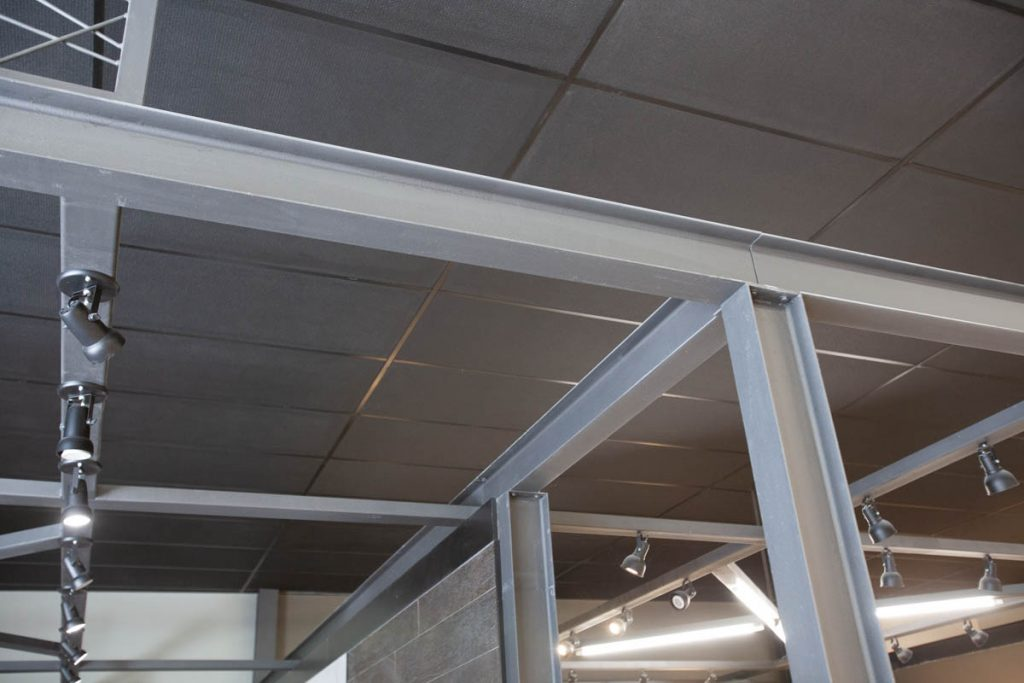
\includegraphics[width=0.5\linewidth]{Imagens/Viga.png}
    \smallcaption{Fonte: RDG Aços do Brasil}
    \label{fig: Estrutura Viga}
 \end{figure}

\section{Elemento de Pórtico}

Os pórticos são elementos formados pela associação de pilares e vigas, ou seja, várias barras situadas em um único plano, com carregamento atuante no mesmo plano do sistema estrutural, que garantem a estabilidade e a resistência a esforços normais, cortantes e de flexão.
Assim como o sistema de vigas, foram adotadas algumas hipóteses simplificadoras durante o desenvolvimento do projeto, tais quais: material isotrópico em regime linear; pequenos deslocamentos; princípio de Saint-Venant; eixo x local conincidente com a linnha neutra; para L/h >=10 podemos considerar cisalhamento desprezivel; seção transversal constante e simétrica; dois nós com 3 graus de liberdade por nó (u, v e theta); Numeração local dos nós = (1,2). 

Ademais, é importante mencionar que para estruturas reais, os carregamentos não são aplicados somente nos nós, ou seja, torna-se necessário a utilização de carregamentos transversais nodais equivalentes para representar esta situação de maneira similar à realidade.

Focalizando nossa análise na ciência dos materiais, os principais recursos utilizados para a construção de pórticos são: concreto armado, aço e madeira. Eles são comumente utilizados em áreas com um espaço amplo e coberto, como fábricas e armazéns, fornecendo uma estrutura forte e resistente que consegue suportar carregamentos de alta magnitude. 
Já no aspecto da engenharia civil, são utilizadas diversas técnicas de análise estrutural que permitem a previsão das cargas máximas exercidas para manter a estrutura segura e com um coeficiente de segurança adequado. Esse processo se comunica diretamente com o estudo dos materiais, necessitando de uma boa seleção de materiais para os pilares e vigas horizontais, bem como o cálculo das forças na estrutura.

\begin{figure}[!htb]
 \centering
    \caption{Exemplo de Estrutura de Pórtico}
    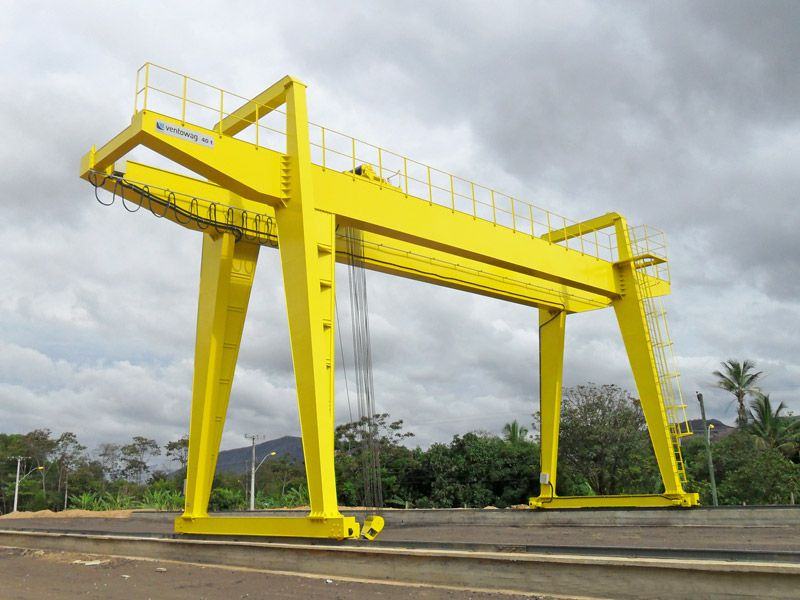
\includegraphics[width=0.6\linewidth]{Imagens/Pórtico.png}
    \smallcaption{Fonte: Treicap}
    \label{fig: Estrutura Portico}
 \end{figure}

\chapter{Projeto}

Neste trecho será apresentado a estrutura escolhida pelo grupo e o código completo para realização da sua análise.

\section{Desenho Esquematizado}

O modelo prático consiste em uma associação de 11 elementos, conforme indicado nas figuras abaixo. O sistema apresenta dois engastamentos, nos nós 7 e 5. 

Utilizamos o Software Autocad para desenvolver e implementar o projeto descrito na Figura [\ref{fig: Estrutura do Projeto}], assim como utilizamos o software MATLAB para analisarmos o deslocamento do sistema com duas forças atuantes distribuidas (15kN/m e 7 kN/m). 

\begin{figure}[!htb]
 \centering
    \caption{Estrutura Base}
    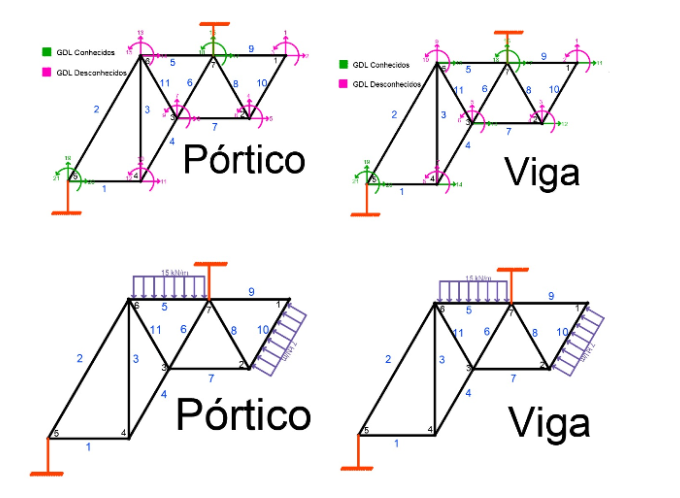
\includegraphics[width=1\linewidth]{Imagens/4Imagens.png}
    \smallcaption{Fonte: Autor}
    \label{fig: Estrutura do Projeto}
 \end{figure}

\section{Códigos}

Os códigos foram desenvolvidos pelo professor Mohammad Shaterzadeh, e adaptados pelo grupo, utilizando o software MATLAB que utiliza a linguagem Fortran. O código utilizado para a simulação está descrito abaixo:

\subsection{Código Principal - Viga}

\begin{lstlisting}
clearvars; clc; close all;

%==============================
% ENTRADA DE DADOS DA ESTRUTURA
%==============================

nEL = 11;         % Quantidade total de elementos
nNO = 7;          % Quantidade total de nós
nGL = 3;          % Quantidade GL por nó

alpha = 1:10 ;    % GLs desconhecidos
beta  = 11:21;    % GLs conhecidos (fixos ou prescritos)

AE = 5;           % *10^5 N
EI = 2;           % *10^6 N/m^2

q1 = 7;          %KN/m
L1 = 2;          % m
q2 = 15;          %KN/m
L2 = 2;          % m
 
% Matriz de tipo de Elemento (ME)
Tipo = [3 3 3 3 3 3 3 3 3 3 3];   % 1 = mola ; 2 = barra; 3 = viga ; 4 = portico
 
% Matriz de Identidade (ID)
ID(1,1:nNO) = [11 12 13 14 20 15 17];
ID(2,1:nNO) = [ 1  3  5  7 19  9 16];
ID(3,1:nNO) = [ 2  4  6  8 21 10 18];

% Matriz de Incidência (IN)
IN(1,1:nEL) = [5 5 4 6 4 3 3 7 7 2 3];
IN(2,1:nEL) = [4 6 6 7 3 7 2 2 1 1 6];

% Matriz de Localização (LM)
LM(1,1:nEL) = [20 20 14 14 15 13 13 12 17 12 13];
LM(2,1:nEL) = [19 19  7  7  9  5  5  3 16  3  5];
LM(3,1:nEL) = [21 21  8  8 10  6  6  4 18  4  6];
LM(4,1:nEL) = [14 15 15 13 17 17 12 17 11 11 15];
LM(5,1:nEL) = [ 7  9  9  5 16 16  3 16  1  1  9];
LM(6,1:nEL) = [ 8 10 10  6 18 18  4 18  2  2 10];

% Matriz de Propriedades (PROP)
PROP(1,1:nEL) = [2  4  3.4641  2   2  2   2   2   2   2   1];
PROP(2,1:nEL) = [0  60   90    0  60  60  0  120  0  60  120];

for n = 1:nEL %LINHA 3
    if Tipo(n) == 1         % 1 = mola
        PROP(3,n) = k;
    elseif Tipo(n) == 2     % 2 = barra
        PROP(3,n) = (AE/PROP(1,n));
    elseif Tipo(n) == 3     % 3 = viga
        PROP(3,n) = nan;
    elseif Tipo(n) == 4     % = portico 
        PROP(3,n) = (AE/PROP(1,n));
    end
end

for n = 1:nEL %LINHA 4
    if Tipo(n) == 1         % 1 = mola
        PROP(4,n) = nan;
    elseif Tipo(n) == 2     % 2 = barra
        PROP(4,n) = nan;
    elseif Tipo(n) == 3     % 3 = viga
        PROP(4,n) = ((12*EI)/(PROP(1,n))^3);
    elseif Tipo(n) == 4     % = portico 
        PROP(4,n) = ((12*EI)/(PROP(1,n))^3) ;
    end
end

for n = 1:nEL %LINHA 5
    if Tipo(n) == 1         % 1 = mola
        PROP(5,n) = nan;
    elseif Tipo(n) == 2     % 2 = barra
        PROP(5,n) = nan;
    elseif Tipo(n) == 3     % 3 = viga
        PROP(5,n) = ((6*EI)/(PROP(1,n))^2);
    elseif Tipo(n) == 4     % = portico 
        PROP(5,n) = ((6*EI)/(PROP(1,n))^2);
    end
end

for n = 1:nEL %LINHA 6
    if Tipo(n) == 1         % 1 = mola
        PROP(6,n) = nan;
    elseif Tipo(n) == 2     % 2 = barra
        PROP(6,n) = nan;
    elseif Tipo(n) == 3     % 3 = viga
        PROP(6,n) = ((2*EI)/(PROP(1,n)));
    elseif Tipo(n) == 4     % = portico 
        PROP(6,n) = ((2*EI)/(PROP(1,n)));
    end
end

% Vetor de carregamentos externos

% Carga 1
F1 = (q1*L1)/2;    % Força aplicada a 1 nó apartir da Força Distruibuida 1 
M1 = (q1*L1^2)/12; % Momento aplicada a 1 nó apartir da Força Distruibuida 1
% Carga 2
F2 = (q2*L2)/2;    % Força aplicada a 1 nó apartir da Força Distruibuida 2 
M2 = (q2*L2^2)/12; % Momento aplicada a 1 nó apartir da Força Distruibuida 2

F = zeros(nNO*nGL,1);
F(alpha) = [(-F1*sind(45)) -M1 (-F1*sind(45)) -M1 0 0 0 0 -F2 -M2]; % Forças conhecidas, referentes aos GLs desconhecidos

% Vetor de graus de liberdade (GLs)
X = zeros(nNO*nGL,1);
X(beta) = [0 0 0 0 0 0 0 0 0 0 0]; % Deslocamento dos GLs conhecidos

% Geometria original ( Considerando o Nó 7 = 0 )
COORD(1,1:nNO) = [  6       5       3      2   0     2      4   ];
COORD(2,1:nNO) = [3.4641 1.73205 1.73205   0   0  3.4641  3.4642];
escala = 0.1;

%==============================
% CÁLCULO DO MEF
%==============================

% Calcula as matriz de rigidez global para cada elemento
for el = 1:nEL
  Ke(:,:,el) = CalculaMatrizRigidezElemento(el,PROP, Tipo);
end

% Monta a matriz de rigidez GLOBAL
Kg = zeros(beta(end));
for el = 1:nEL
    if or(Tipo(el) == 1, Tipo(el) == 2) % Mola e Barra
        Kg(LM(1:4,el),LM(1:4,el))=Kg(LM(1:4,el),LM(1:4,el))+Ke(1:4,1:4,el);
    elseif or (Tipo(el) == 3,Tipo(el) == 4) %Viga e Portico
        Kg(LM(:,el),LM(:,el))=Kg(LM(:,el),LM(:,el))+Ke(:,:,el);
    end       
end

% Verifica se a solução existe e é única
det(Kg(alpha,alpha));   % É diferente de zero -> OK! 

% Solução dos GLs desconhecidos
X(alpha) = Kg(alpha,alpha)\(F(alpha)-Kg(alpha,beta)*X(beta));

% Cálculo das reações de apoio
F(beta) = Kg(beta,alpha)*X(alpha) + Kg(beta,beta)*X(beta);

% Verificação das condições de equilíbrio
Fx = F(1:2:end);
sum(Fx);  
Fy = F(2:2:end);
sum(Fy);

% Cálculo da energia potencial
for el = 1 : nEL
    if or(Tipo(el) == 1, Tipo(el) == 2)
        Xel = X(LM(1:4,el));
        U(el) = .5*Xel'*Ke(1:4,1:4,el)*Xel;
    elseif or (Tipo(el) == 3,Tipo(el) == 4)
        Xel = X(LM(:,el));
        U(el) = .5*Xel'*Ke(:,:,el)*Xel;
    end
end

% Cálculo das forças nos elementos
for el = 1 : nEL
  if or(Tipo(el) == 1, Tipo(el) == 2) %Mola e Barra
        Ke_local = PROP(3,el)*[ 1 0 -1 0; 0 0 0 0;...
                               -1 0  1 0; 0 0 0 0];
        T = CalculaMatrizTransformacao(el,PROP,Tipo);
        Xel = X(LM(1:4,el));
        Xel_local = T * Xel;
        Felem(1:4,el) = Ke_local * Xel_local;
  elseif Tipo(el) == 3 %Viga
          Ke_local = [ 0 0 0 0 0 0; 0 PROP(4,el) PROP(5,el) 0 -PROP(4,el) PROP(5,el);
                       0 PROP(5,el) 2*PROP(6,el) 0 -PROP(5,el) PROP(6,el); 0 0 0 0 0 0;
                       0 -PROP(4,el) -PROP(5,el) 0 PROP(5,el) PROP(4,el); 0 PROP(4,el) PROP(6,el) 0 -PROP(4,el) 2*PROP(6,el)];
        T = CalculaMatrizTransformacao(el,PROP,Tipo);
        Xel = X(LM(:,el));
        Xel_local = T * Xel;
        Felem(:,el) = Ke_local * Xel_local;
  elseif Tipo(el) == 4 %Portico
          Ke_local = [ PROP(3,el) 0 0 -PROP(3,el) 0 0; 0 PROP(4,el) PROP(5,el) 0 -PROP(4,el) PROP(5,el);
                       0 PROP(5,el) 2*PROP(6,el) 0 -PROP(5,el) PROP(6,el); -PROP(3,el) 0 0 PROP(3,el) 0 0;
                       0 -PROP(4,el) -PROP(5,el) 0 PROP(5,el) PROP(4,el); 0 PROP(4,el) PROP(6,el) 0 -PROP(4,el) 2*PROP(6,el)];
        T = CalculaMatrizTransformacao(el,PROP,Tipo);
        Xel = X(LM(:,el));
        Xel_local = T * Xel;
        Felem(:,el) = Ke_local * Xel_local;
  end
end

%==============================
% PLOTAGEM
%==============================

figure(1); hold on;
% Plota os nós
for i = 1 : nNO
  plot(COORD(1,i), COORD(2,i), 'bo');
end
box on; grid on; axis equal;
% Plota os elementos
for el = 1 : nEL
  plot(COORD(1,IN(:,el)),COORD(2,IN(:,el)),'b--','DisplayName','Original');
end

% Geometria deformada
DEF(1,:) = COORD(1,:) + escala*X(ID(1,:))';
DEF(2,:) = COORD(2,:) + escala*X(ID(2,:))';

% Plota os nós deslocados
for i = 1 : nNO
  plot(DEF(1,i), DEF(2,i), 'ro');
end
box on; grid on; axis equal;
% Plota os elementos deformados
for el = 1 : nEL
  plot(DEF(1,IN(:,el)),DEF(2,IN(:,el)),'r','linewidth',3,'DisplayName','Deformada');
end

title('GEOMETRIA ORIGINAL E DEFORMADA - VIGA','Fontsize',20);

\end{lstlisting}

\subsection{Código Principal - Pórtico}

\begin{lstlisting}
clearvars; clc; close all;

%==============================
% ENTRADA DE DADOS DA ESTRUTURA
%==============================

nEL = 11;         % Quantidade total de elementos
nNO = 7;          % Quantidade total de nós
nGL = 3;          % Quantidade GL por nó

alpha = 1:15 ;    % GLs desconhecidos
beta  = 16:21;    % GLs conhecidos (fixos ou prescritos)

AE = 5;           % *10^5 N
EI = 2;           % *10^6 N/m^2

q1 = 7;          %KN/m
L1 = 2;          % m
q2 = 15;          %KN/m
L2 = 2;          % m

% Matriz de tipo de Elemento (ME)
Tipo = [4 4 4 4 4 4 4 4 4 4 4];   % 1 = mola ; 2 = barra; 3 = viga ; 4 = portigo
 
% Matriz de Identidade (ID)
ID(1,1:nNO) = [2 5 8 11 20 14 17];
ID(2,1:nNO) = [1 4 7 10 19 13 16];
ID(3,1:nNO) = [3 6 9 12 21 15 18];

% Matriz de Incidência (IN)
IN(1,1:nEL) = [5 5 4 6 4 3 3 7 7 2 3];
IN(2,1:nEL) = [4 6 6 7 3 7 2 2 1 1 6];

% Matriz de Localização (LM)
LM(1,1:nEL) = [20  20  11 11 14  8 8 5 17 5  6];
LM(2,1:nEL) = [19  19  10 10 13  7 7 4 16 4  7];
LM(3,1:nEL) = [21  21  12 12 15  9 9 6 18 6  9];
LM(4,1:nEL) = [11  14  14  8 17 17 5 17 2 2 14];
LM(5,1:nEL) = [10  13  13  7 16 16 4 16 1 1 13];
LM(6,1:nEL) = [12  15  15  9 18 18 6 18 3 3 15];

% Matriz de Propriedades (PROP)
PROP(1,1:nEL) = [2  4  3.4641  2   2  2   2   2   2   2   1];
PROP(2,1:nEL) = [0  60   90    0  60  60  0  120  0  60  120];

for n = 1:nEL %LINHA 3
    if Tipo(n) == 1         % 1 = mola
        PROP(3,n) = k;
    elseif Tipo(n) == 2     % 2 = barra
        PROP(3,n) = (AE/PROP(1,n));
    elseif Tipo(n) == 3     % 3 = viga
        PROP(3,n) = nan;
    elseif Tipo(n) == 4     % = portico 
        PROP(3,n) = (AE/PROP(1,n));
    end
end

for n = 1:nEL %LINHA 4
    if Tipo(n) == 1         % 1 = mola
        PROP(4,n) = nan;
    elseif Tipo(n) == 2     % 2 = barra
        PROP(4,n) = nan;
    elseif Tipo(n) == 3     % 3 = viga
        PROP(4,n) = ((12*EI)/(PROP(1,n))^3);
    elseif Tipo(n) == 4     % = portico 
        PROP(4,n) = ((12*EI)/(PROP(1,n))^3) ;
    end
end

for n = 1:nEL %LINHA 5
    if Tipo(n) == 1         % 1 = mola
        PROP(5,n) = nan;
    elseif Tipo(n) == 2     % 2 = barra
        PROP(5,n) = nan;
    elseif Tipo(n) == 3     % 3 = viga
        PROP(5,n) = ((6*EI)/(PROP(1,n))^2);
    elseif Tipo(n) == 4     % = portico 
        PROP(5,n) = ((6*EI)/(PROP(1,n))^2);
    end
end

for n = 1:nEL %LINHA 6
    if Tipo(n) == 1         % 1 = mola
        PROP(6,n) = nan;
    elseif Tipo(n) == 2     % 2 = barra
        PROP(6,n) = nan;
    elseif Tipo(n) == 3     % 3 = viga
        PROP(6,n) = ((2*EI)/(PROP(1,n)));
    elseif Tipo(n) == 4     % = portico 
        PROP(6,n) = ((2*EI)/(PROP(1,n)));
    end
end

% Vetor de carregamentos externos

% Carga 1
F1 = (q1*L1)/2;    % Força aplicada a 1 nó apartir da Força Distruibuida 1 
M1 = (q1*L1^2)/12; % Momento aplicada a 1 nó apartir da Força Distruibuida 1
% Carga 2
F2 = (q2*L2)/2;    % Força aplicada a 1 nó apartir da Força Distruibuida 2 
M2 = (q2*L2^2)/12; % Momento aplicada a 1 nó apartir da Força Distruibuida 2

F = zeros(nNO*nGL,1);
F(alpha) = [(-F1*cosd(45)) (-F1*sind(45)) -M1 (-F1*cosd(45)) (-F1*sind(45)) -M1 0 0 0 0 0 0 -F2 -F2 -M2]; % Forças conhecidas, referentes aos GLs desconhecidos

% Vetor de graus de liberdade (GLs)
X = zeros(nNO*nGL,1);
X(beta) = [0 0 0 0 0 0]; % Deslocamento dos GLs conhecidos

% Geometria original ( Considerando o Nó 7 = 0 )
COORD(1,1:nNO) = [  6       5       3      2   0     2      4   ];
COORD(2,1:nNO) = [3.4641 1.73205 1.73205   0   0  3.4641  3.4642];
escala = 0.1;

%==============================
% CÁLCULO DO MEF
%==============================

% Calcula as matriz de rigidez global para cada elemento
for el = 1:nEL
  Ke(:,:,el) = CalculaMatrizRigidezElemento(el,PROP, Tipo);
end

% Monta a matriz de rigidez GLOBAL
Kg = zeros(beta(end));
for el = 1:nEL
    if or(Tipo(el) == 1, Tipo(el) == 2) % Mola e Barra
        Kg(LM(1:4,el),LM(1:4,el))=Kg(LM(1:4,el),LM(1:4,el))+Ke(1:4,1:4,el);
    elseif or (Tipo(el) == 3,Tipo(el) == 4) %Viga e Portico
        Kg(LM(:,el),LM(:,el))=Kg(LM(:,el),LM(:,el))+Ke(:,:,el);
    end       
end

% Verifica se a solução existe e é única
det(Kg(alpha,alpha));   % É diferente de zero -> OK! 

% Solução dos GLs desconhecidos
X(alpha) = Kg(alpha,alpha)\(F(alpha)-Kg(alpha,beta)*X(beta));

% Cálculo das reações de apoio
F(beta) = Kg(beta,alpha)*X(alpha) + Kg(beta,beta)*X(beta);

% Verificação das condições de equilíbrio
Fx = F(1:2:end);
sum(Fx);  
Fy = F(2:2:end);
sum(Fy);

% Cálculo da energia potencial
for el = 1 : nEL
    if or(Tipo(el) == 1, Tipo(el) == 2)
        Xel = X(LM(1:4,el));
        U(el) = .5*Xel'*Ke(1:4,1:4,el)*Xel;
    elseif or (Tipo(el) == 3,Tipo(el) == 4)
        Xel = X(LM(:,el));
        U(el) = .5*Xel'*Ke(:,:,el)*Xel;
    end
end

% Cálculo das forças nos elementos
for el = 1 : nEL
  if or(Tipo(el) == 1, Tipo(el) == 2) %Mola e Barra
        Ke_local = PROP(3,el)*[ 1 0 -1 0; 0 0 0 0;...
                               -1 0  1 0; 0 0 0 0];
        T = CalculaMatrizTransformacao(el,PROP,Tipo);
        Xel = X(LM(1:4,el));
        Xel_local = T * Xel;
        Felem(1:4,el) = Ke_local * Xel_local;
  elseif Tipo(el) == 3 %Viga
          Ke_local = [ 0 0 0 0 0 0; 0 PROP(4,el) PROP(5,el) 0 -PROP(4,el) PROP(5,el);
                       0 PROP(5,el) 2*PROP(6,el) 0 -PROP(5,el) PROP(6,el); 0 0 0 0 0 0;
                       0 -PROP(4,el) -PROP(5,el) 0 PROP(5,el) PROP(4,el); 0 PROP(4,el) PROP(6,el) 0 -PROP(4,el) 2*PROP(6,el)];
        T = CalculaMatrizTransformacao(el,PROP,Tipo);
        Xel = X(LM(:,el));
        Xel_local = T * Xel;
        Felem(:,el) = Ke_local * Xel_local;
  elseif Tipo(el) == 4 %Portico
          Ke_local = [ PROP(3,el) 0 0 -PROP(3,el) 0 0; 0 PROP(4,el) PROP(5,el) 0 -PROP(4,el) PROP(5,el);
                       0 PROP(5,el) 2*PROP(6,el) 0 -PROP(5,el) PROP(6,el); -PROP(3,el) 0 0 PROP(3,el) 0 0;
                       0 -PROP(4,el) -PROP(5,el) 0 PROP(5,el) PROP(4,el); 0 PROP(4,el) PROP(6,el) 0 -PROP(4,el) 2*PROP(6,el)];
        T = CalculaMatrizTransformacao(el,PROP,Tipo);
        Xel = X(LM(:,el));
        Xel_local = T * Xel;
        Felem(:,el) = Ke_local * Xel_local;
  end
end

%==============================
% PLOTAGEM
%==============================

figure(1); hold on;
% Plota os nós
for i = 1 : nNO
  plot(COORD(1,i), COORD(2,i), 'bo');
end
box on; grid on; axis equal;
% Plota os elementos
for el = 1 : nEL
  plot(COORD(1,IN(:,el)),COORD(2,IN(:,el)),'b--','DisplayName','Original');
end

% Geometria deformada
DEF(1,:) = COORD(1,:) + escala*X(ID(1,:))';
DEF(2,:) = COORD(2,:) + escala*X(ID(2,:))';

% Plota os nós deslocados
for i = 1 : nNO
  plot(DEF(1,i), DEF(2,i), 'ro');
end
box on; grid on; axis equal;
% Plota os elementos deformados
for el = 1 : nEL
  plot(DEF(1,IN(:,el)),DEF(2,IN(:,el)),'r','linewidth',3,'DisplayName','Deformada');
end

title('GEOMETRIA ORIGINAL E DEFORMADA - PORTICO','Fontsize',20);


\end{lstlisting}

\subsection{Cálculo da Matriz de Rigidez dos Elemento}

\begin{lstlisting}
function Ke = CalculaMatrizRigidezElemento(el,PROP,Tipo)

m = cosd(PROP(2,el));
n = sind(PROP(2,el));
fi = PROP(4,el);
lb = PROP(5,el);
ro = PROP(6,el);

    if or(Tipo(el) == 1, Tipo(el) == 2)     %Mola e Barra 
        Ke = PROP(3,el)*[ m^2  m*n -m^2 -m*n 0 0;
                          m*n  n^2 -m*n -n^2 0 0;
                         -m^2 -m*n  m^2  m*n 0 0;
                         -m*n -n^2  m*n  n^2 0 0;
                          0     0    0    0  0 0;
                          0     0    0    0  0 0 ];
        
    elseif Tipo(el) == 3                     %Viga 
        Ke = [ fi*n^2  -fi*m*n   -lb*n  -fi*n^2  fi*m*n -lb*n;
              -fi*m*n   fi*m^2    lb*m   fi*m*n -fi*m^2  lb*m;
              -lb*n     lb*m      2*ro   lb*n   -lb*m    ro;
              -fi*n^2   fi*m*n    lb*n   fi*n^2 -fi*m*n  lb*n;
               fi*m*n  -fi*m^2   -lb*m  -fi*m*n  fi*m^2 -lb*m;
              -lb*n     lb*m       ro    lb*n   -lb*m    2*ro ];

    elseif Tipo(el) == 4                     %Portico
        Ke1 = PROP(3,el)*[    m^2  m*n  0 -m^2 -m*n 0;
                              m*n  n^2  0 -m*n -n^2 0
                              0     0   0   0    0  0;
                             -m^2 -m*n  0  m^2  m*n 0;
                             -m*n -n^2  0  m*n  n^2 0;
                              0     0   0   0    0  0   ];

        Ke2 = [fi*n^2  -fi*m*n   -lb*n  -fi*n^2  fi*m*n -lb*n;
              -fi*m*n   fi*m^2    lb*m   fi*m*n -fi*m^2  lb*m;
               lb*n     lb*m      2*ro   lb*n   -lb*m    ro;
              -fi*n^2   fi*m*n    lb*n   fi*n^2 -fi*m*n  lb*n;
               fi*m*n  -fi*m^2   -lb*m  -fi*m*n  fi*m^2 -lb*m;
              -lb*n     lb*m       ro    lb*n   -lb*m    2*ro ];

        Ke = Ke1 + Ke2;
    end

\end{lstlisting}


\subsection{Cálculo da Matriz de Transformação}

\begin{lstlisting}
function T = CalculaMatrizTransformacao(el,PROP,Tipo)

% Matriz Transformação
m = cosd(PROP(2,el));
n = sind(PROP(2,el));

if or(Tipo(el) == 1, Tipo(el) == 2)     %Mola e Barra 

       T = [ m n  0 0;
            -n m  0 0;
             0 0  m n;
             0 0 -n m];
      
    elseif or(Tipo(el) == 3,Tipo(el) == 4 ) %Viga e Pórtico

        T = [ m n 0  0 0 0
             -m m 0  0 0 0
              0 0 1  0 0 0 
              0 0 0  m n 0
              0 0 0 -n m 0
              0 0 0  0 0 1];
end     
      
\end{lstlisting}

\chapter{Montagem das Matrizes}

\section{Matrizes de Identidade (ID)}

\begin{table}[!hb]
 \centering
    \caption{Matriz de Identidade (ID), para Vigas}
    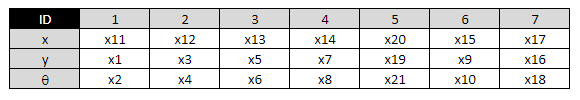
\includegraphics[width=0.8\linewidth]{Tabelas/10Matriz de Identidade (V).png}
    \smallcaption{Fonte: Autor}
    \label{tab: Matriz ID Viga}
 \end{table}

 \begin{table}[!hb]
 \centering
    \caption{Matriz de Identidade (ID), para Pórticos}
    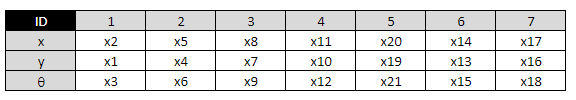
\includegraphics[width=0.8\linewidth]{Tabelas/11Matriz de Identidade (P).png}
    \smallcaption{Fonte: Autor}
    \label{tab: Matriz ID Portico}
 \end{table}    

Para preencher ambas as Matrizes de Identidade (ID), que estão indicadas nas Tabelas  [\ref{tab: Matriz ID Viga}] e [\ref{tab: Matriz ID Portico}], foi necessário definir quais são os graus de liberdade verticais, horizontais e angulados, assim como indicado nas Figuras [\ref{fig: Estrutura ID Viga}] e [\ref{fig: Estrutura ID Portico}].

 \begin{figure}[!htb]
 \centering
    \caption{Estrutura e seus Graus de Liberdade, para Viga.}
    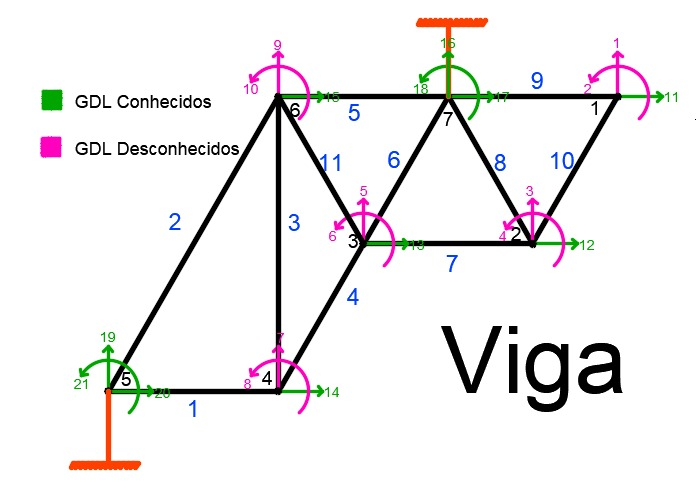
\includegraphics[width=0.75\linewidth]{Imagens/Estrutura ID (V).jpeg}
    \smallcaption{Fonte: Autor}
    \label{fig: Estrutura ID Viga}
 \end{figure}

\begin{figure}[!htb]
 \centering
    \caption{Estrutura e seus Graus de Liberdade, para Pórtico.}
    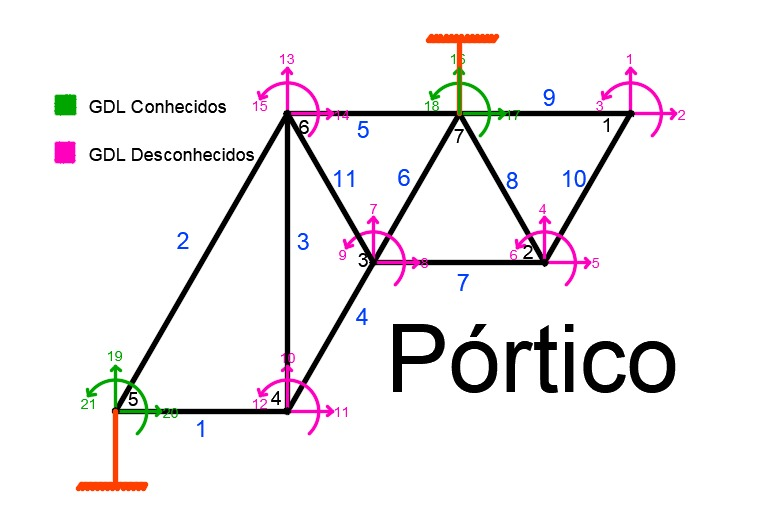
\includegraphics[width=0.75\linewidth]{Imagens/Estrutura ID (P).jpeg}
    \smallcaption{Fonte: Autor}
    \label{fig: Estrutura ID Portico}
 \end{figure}

\section{Matriz de Localização (LM)}

\begin{table}[!htb]
 \centering
    \caption{Matriz de Localização (LM), para Viga.}
    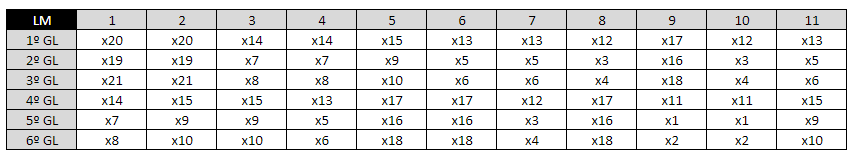
\includegraphics[width=1\linewidth]{Tabelas/12Matriz de Localização (V).png}
    \smallcaption{Fonte: Autor}
    \label{tab: Matriz LM Viga}
 \end{table}

\begin{table}[!htb]
 \centering
    \caption{Matriz de Localização (LM), para Pórtico.}
    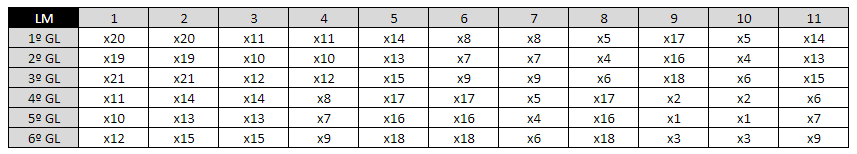
\includegraphics[width=1\linewidth]{Tabelas/13Matriz de Localização (P).png}
    \smallcaption{Fonte: Autor}
    \label{tab: Matriz LM Portico}
 \end{table}
 
Para preencher as Matrizes de Localização (LM), que estão indicadas nas Tabelas [\ref{tab: Matriz LM Viga}] e [\ref{tab: Matriz LM Portico}], foi necessário definir quais são os graus de liberdade verticais, horizontais e angulados de um primeiro nó, e os mesmos parâmetros de um segundo nó, representando assim o elemento entre estes dois pontos escolhidos, assim como indicado nas Figuras [\ref{fig: Estrutura LM Viga}] e [\ref{fig: Estrutura LM Portico}].

\begin{figure}[!htb]
 \centering
    \caption{Estrutura e seus Graus de Liberdade Totais, para Viga.}
    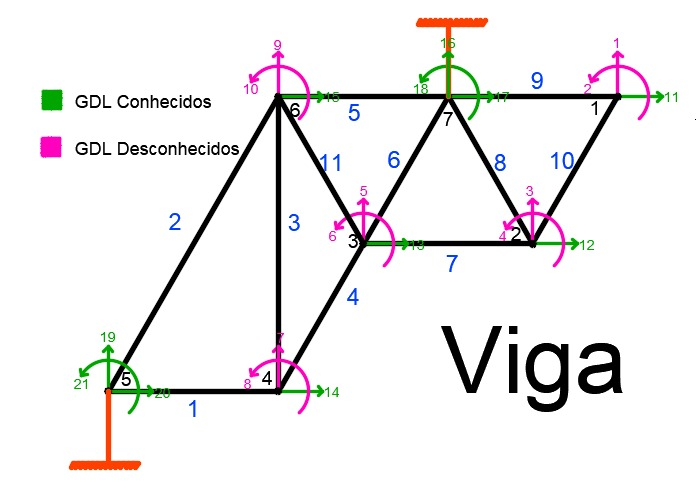
\includegraphics[width=0.7\linewidth]{Imagens/Estrutura ID (V).jpeg}
    \smallcaption{Fonte: Autor}
    \label{fig: Estrutura LM Viga}
 \end{figure}

 \begin{figure}[!htb]
 \centering
    \caption{Estrutura e seus Graus de Liberdade Totais, para Pórtico.}
    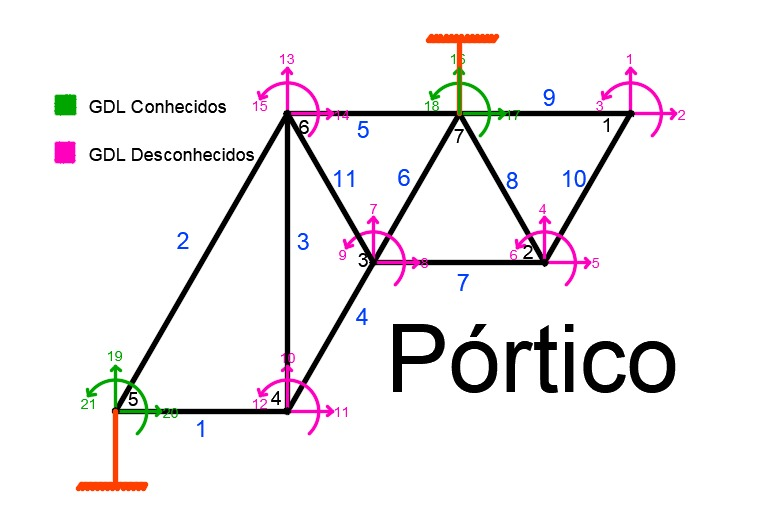
\includegraphics[width=0.7\linewidth]{Imagens/Estrutura ID (P).jpeg}
    \smallcaption{Fonte: Autor}
    \label{fig: Estrutura LM Portico}
 \end{figure}

\section{Matriz de Incidência (IN)}

\begin{table}[!htb]
 \centering
    \caption{Matriz de Incidência (IN).}
    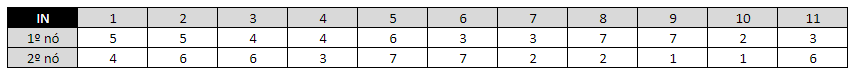
\includegraphics[width=1\linewidth]{Tabelas/14Matriz de Incidencia.png}
    \smallcaption{Fonte: Autor}
    \label{tab: Matriz IN}
 \end{table}
 
Preenchemos a Matriz de Incidência (IN), que está indicada na Tabela [\ref{tab: Matriz IN}], representando um elemento de rigidez. Através da posição de um nó inicial, até um nó final, é possível indicar a posição deste elemento, assim como indicado na Figura [\ref{fig: Estrutura IN}].

\begin{figure}[!htb]
 \centering
    \caption{Elementos e Nós.}
    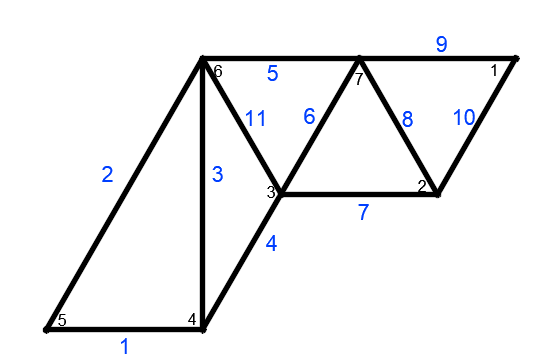
\includegraphics[width=0.75\linewidth]{Imagens/Estrutura IN.png}
    \smallcaption{Fonte: Autor}
    \label{fig: Estrutura IN}
 \end{figure}
 
\section{Matriz de Propriedades (PROP)}

\begin{table}[!htb]
 \centering
    \caption{Matriz de Proppreidades (PROP), para Vigas.}
    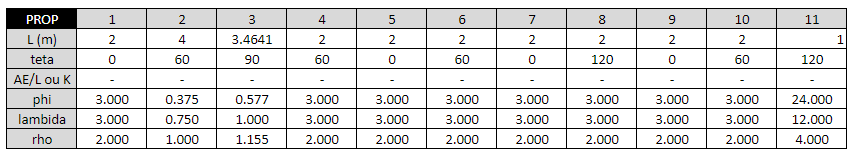
\includegraphics[width=1\linewidth]{Tabelas/15Matriz de Propriedades (V).png}
    \smallcaption{Fonte: Autor}
    \label{tab: Matriz PROP Viga}
 \end{table}

 \begin{table}[!htb]
 \centering
    \caption{Matriz de Proppreidades (PROP), para Pórtico.}
    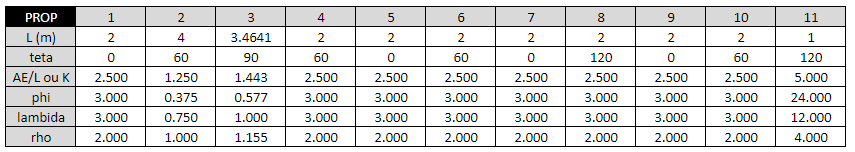
\includegraphics[width=1\linewidth]{Tabelas/16Matriz de Propriedades (P).png}
    \smallcaption{Fonte: Autor}
    \label{tab: Matriz PROP Portico}
 \end{table}

Para preencher as Matrizes de Propriedades (PROP), que estão indicadas nas Tabelas [\ref{tab: Matriz PROP Viga}] e [\ref{tab: Matriz PROP Portico}], foi necessário definir o ângulo entre uma referência horizontal X, até um elemento de rigidez, adotando sempre o sentido anti-horário, assim como indicado na Figura [\ref{fig: Estrutura PROP}].

\begin{figure}[!htb]
 \centering
    \caption{Angulo dos Elementos.}
    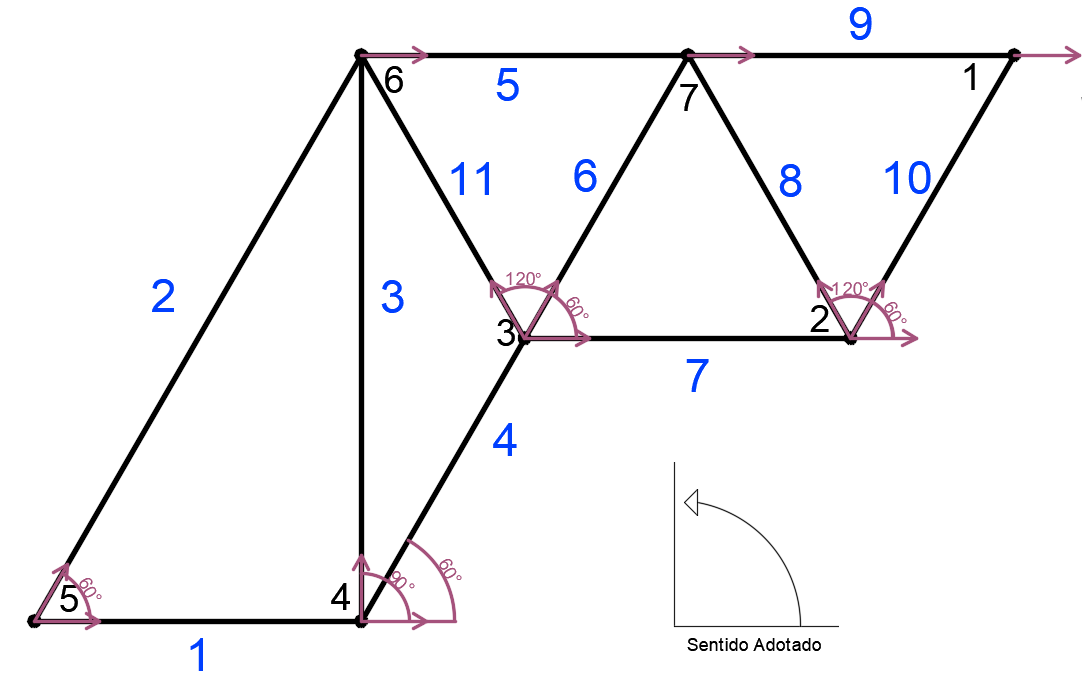
\includegraphics[width=0.7\linewidth]{Imagens/Estrutura PROP.png}
    \smallcaption{Fonte: Autor}
    \label{fig: Estrutura PROP}
 \end{figure}
 
\section{Matriz de Coordenadas (COORD)}

\begin{table}[!htb]
    \centering
    \caption{Matriz de Coordenadas (COORD).}
    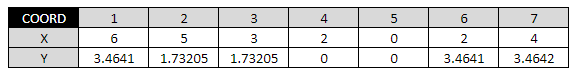
\includegraphics[width=0.9\linewidth]{Tabelas/9Matriz de Coordenada.png}
    \smallcaption{Fonte: Autor}
    \label{tab: Matriz COORD}
 \end{table}

Para preencher a Matriz de Coordenas (COORD), que está indicada na Tabela [\ref{tab: Matriz COORD}], foi necessário escolher um plano cartesiano qualquer, com um ponto referencial (0;0), ou seja X=0 e Y=0, e medir a distancia em X e Y de todos os nós em relação a este referencial. Assim como indicado na Figura [\ref{fig: Estrutura COORD}].

\begin{figure}[ht]
   \centering
    \caption{Coordenadas dos Nós.}
    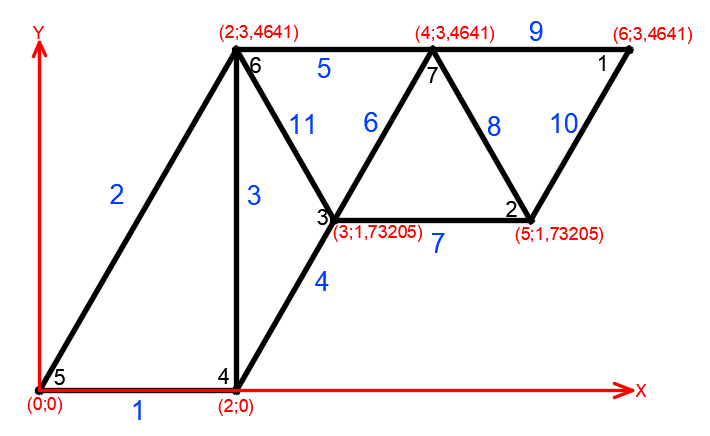
\includegraphics[width=0.8\linewidth]{Imagens/Estrutura CORD.png}
    \smallcaption{Fonte: Autor}
    \label{fig: Estrutura COORD}
 \end{figure}

\chapter{Resultado e Discussão}

Nesse trecho será feita uma breve análise sobre as matrizes de saídas do código, no caso, as matrizes de força, deformação e energia potencial. Além disso, faremos apontamentos sobre o resultado final do experimento, comentando a respeito do gráfico da geometria deformada.

\section{Forças aplicadas}


\begin{table}[!htb]
 \centering
    \caption{Forças Aplicadas Pórtico.}
    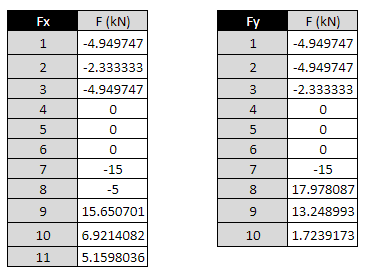
\includegraphics[width=0.6\linewidth]{Tabelas/3Forças Aplicadas (P).png}
    \smallcaption{Fonte: Autor}
    \label{tab: Forças aplicadas Portico}
\end{table}

\begin{table}[!htb]
 \centering
    \caption{Forças Aplicadas Viga.}
    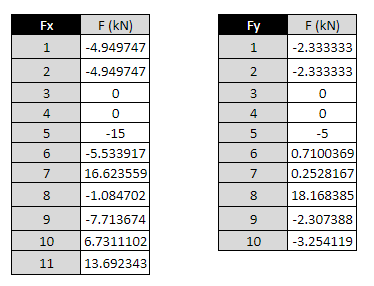
\includegraphics[width=0.6\linewidth]{Tabelas/4Forças Aplicadas (V).png}
    \smallcaption{Fonte: Autor}
    \label{tab: Forças aplicadas Viga}
 \end{table}
 
Primeiramente obtivemos através do MATLAB a Matriz de Forças [\ref{tab: Forças aplicadas Portico}] e [\ref{tab: Forças aplicadas Viga}] no eixo X e Y em cada elemento de nossa estrutura, foi possível observar que os elementos com uma maior concentração de forças aplicadas foram os 8º e 9º elementos para pórtico e os 7º e o 8º para viga e .

\section{Forças nos elementos}

\begin{table}[!htb]
 \centering
    \caption{Forças Aplicadas para Viga e Pórtico.}
    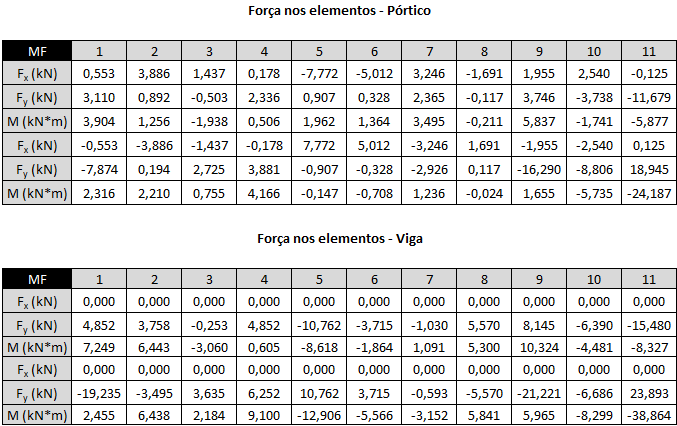
\includegraphics[width=1\linewidth]{Tabelas/TabelaForças.png}
    \smallcaption{Fonte: Autor}
    \label{tab: Forças nos elementos}
\end{table}

Obtivemos também a Matriz de Forças em Cada Elemento do Sistema [\ref{tab: Forças nos elementos}], sendo estas referentes as coordenadas locais, nos permitindo apontar que os elementos que tem maior força concentrada são os elementos 11, 5  em Pórtico e 11, 5 em Viga. Nenhum elemento em Viga  apresenta Forças no eixo X pois seria caracterizado como Compressão, algo que o sistema não apresenta.

\section{Deformações}

\begin{figure}[!ht]
 \centering
    \caption{Gráficos das Deformações.}
    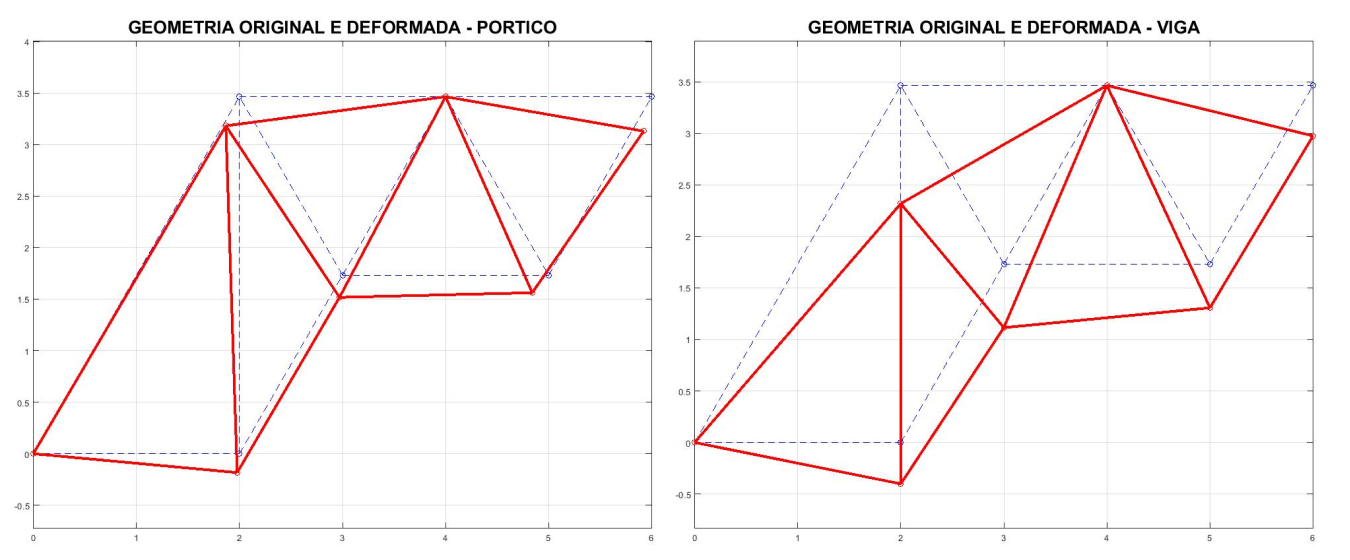
\includegraphics[width=1\linewidth]{Imagens/DeformaçãoTotal.png}
    \smallcaption{Fonte: Autor}
    \label{fig: Deformação}
 \end{figure}

A partir dos Gráficos [\ref{fig: Deformação}] retirado do MATLAB, foi possível observar como seria a deformação de nossa estrutura com as forças definidas, isso é de grande ajuda para ter uma melhor visualização do projeto, nos permitindo ter uma ideia geral de como seriam esses deslocamentos, tendo maior facilidade do que na análise por tabelas.
 
\begin{table}[!htb]
 \centering
    \caption{Matriz de Deformações.}
    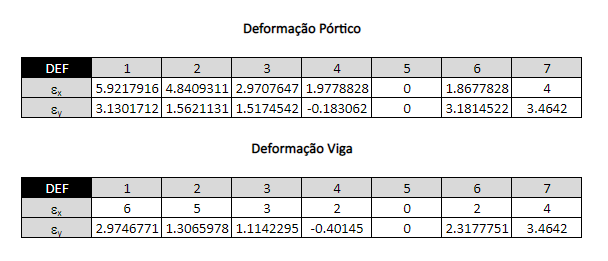
\includegraphics[width=1\linewidth]{Tabelas/TabelaDeformações.png}
    \smallcaption{Fonte: Autor}
    \label{tab: Deformormação}
 \end{table}

Foi retirada do MATLAB as Matrizes das Deformações em cada nó da Estrutura [\ref{tab: Deformormação}], que ao observarmos podemos analisar que os pontos que sofreram a maior deformação no eixo X e Y, respectivamente, foram o 1º e 7º, tanto para viga quanto para pórtico. 

\section{Energia Potencial}

\begin{table}[!htb]
 \centering
    \caption{Matriz Cálculo da Energia Potencial.}
    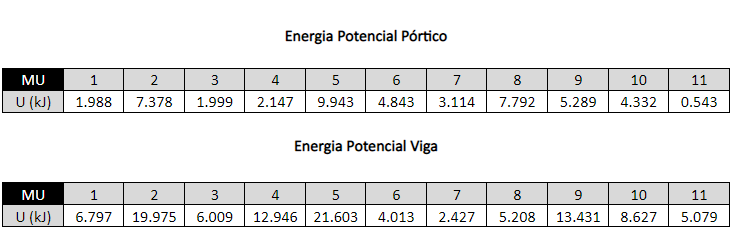
\includegraphics[width=1\linewidth]{Tabelas/TabelaEnergiaPotencial.png}
    \smallcaption{Fonte: Autor}
    \label{tab: Energia Potencial}
 \end{table}

Ao longo de nosso experimento também calculamos a Energia Potencial em cada elemento de nossa estrutura [\ref{tab: Energia Potencial}], possibilitando analisarmos a distribuição e concentração de energia potencial, onde os elementos que apresentaram maior energia potencial foram 2, 5 e 8.
 
\chapter{Conclusão}

Diante dos dados supra-apresentados, torna-se notável a grande importancia de estudar o comportamento de pórtico e viga, afim de saber a estabilidade, força e deslocamento suportados por eles. Em uma situação real essa análise poderia levar a uma melhor compreensão do problema estudado, otimizando dessa maneira os processos produtivos e construtivos, evitando qualquer tipo de desperdício desnecessário. Ademais, é importante ressaltar que com o auxílio dos softwares utilizados (MatLAB, Excel e AutoCAD), e com os ensinamentos adquiridos durante o semestre, se tornou possível realizar esta analise completa obtendo os resultados desejados, e concluir que os mesmos são fidedignos aos resultados esperados para esse componente. 

\printbibliography[type=online]
\nocite{*}

\end{document}